\chapter{Introduction} 
%
% This line creates a new chapter titled "Introduction" in the document. 
% The 'chapter' command automatically numbers the chapter and starts it on a new page.
%
% 1.1
{ \textbf{1.1 {Object Detection}}}\newline
\newline
%
% This creates a bolded heading for section "1.1 Object Detection". 
% The '\newline' ensures a line break after the title. The double '\newline' introduces a gap between the title and the content.
%
Object detection is a fundamental task in the field of computer vision, involving both the identification and localization of objects within images or video sequences. Unlike image classification, which assigns a single label to an entire image, object detection aims to detect multiple objects in an image by predicting their class labels and precisely locating them using bounding boxes.\newline
\\
% This paragraph introduces the concept of object detection and explains how it differs from image classification.
% '\newline' and '\\' are used to create line breaks and separate the content.
%
\begin{figure}[h!] 
    \centering
    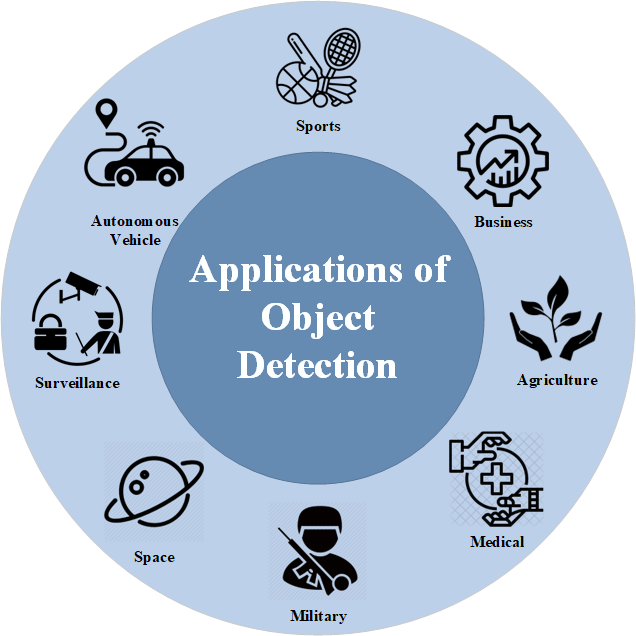
\includegraphics[width=0.5\textwidth]{images/Object Detection Application.png}
    \caption{Applications of Object Detection Methods}
  \end{figure}
\\\\
% This block inserts a figure displaying the applications of object detection methods.
% The '[h!]' option tells LaTeX to try and place the figure "here" (at the current location).
% '\centering' centers the figure horizontally on the page.
% The image file is inserted using '\includegraphics', and the 'width' option scales it to 30% of the page width.
% '\caption' adds a description below the figure.
%
Object detection has become an essential component in many real-world applications, including:
% This sentence introduces a list of real-world applications where object detection is crucial.
%
\begin{itemize}
  \item \textbf{Surveillance Systems and Public Safety:} Object detection is widely used in monitoring public spaces for security purposes, detecting potential threats or suspicious activities in real-time.
  \item \textbf{Autonomous Vehicles and Traffic Management:} In self-driving cars, object detection helps identify road elements such as pedestrians, vehicles, and traffic signs, enabling safe navigation and collision avoidance.
  \item \textbf{Robotics:} By incorporating object detection, robots can interact with their surroundings, such as grasping objects or navigating through obstacles.
  \item \textbf{Medical Imaging:} Object detection aids medical professionals in diagnosing diseases by identifying abnormalities such as tumors or lesions in medical images.
  \item \textbf{Industrial Automation:} Object detection plays a critical role in automating tasks like quality control, defect detection, and monitoring production lines in manufacturing industries.
  \\
\end{itemize}
% This block creates an itemized list of applications for object detection, with each application highlighted in bold.
% '\item' introduces each new item in the list.
% The double '\\' introduces extra spacing after the list.
%
% 1.2
{ \textbf{1.2 {Object Detection Methods}}}
\\
% This creates a new bolded heading for section "1.2 Object Detection Methods".
% The '\\' forces a line break after the title.
%
\begin{itemize}
  \item[\textbf{A.}] \textbf{Traditional Object Detection Methods}\\\\ 
  % This creates the first item in the list with a subheading "A. Traditional Object Detection Methods" in bold.
  % Double '\\' adds extra spacing before the list of methods.
  %  
  Earlier object detection approaches rely on hand-crafted features and image processing techniques. Notable traditional methods include:
  \begin{itemize}
    \item \textbf{Viola-Jones Algorithm:} Known for its speed and efficiency, this algorithm uses Haar-like features and a cascade classifier to detect objects, particularly faces.
    \item \textbf{Histogram of Oriented Gradients (HOG):} HOG works by analyzing the gradient orientations in localized portions of an image and is commonly used for pedestrian detection.
    \item \textbf{Deformable Parts Model (DPM):} DPM treats objects as collections of deformable parts, using a sliding window approach to detect objects based on part configurations.\\
  \end{itemize}
  % This nested list introduces traditional object detection methods (Viola-Jones, HOG, DPM), with brief descriptions of each. 
  % '\item' and '\textbf' are used to create each bolded item with corresponding details.
  % '\\' adds extra spacing before the list of methods.
  %
  \item[\textbf{B.}] \textbf{Deep Learning-Based Object Detection Methods}\\\\
  % This is another item in the list with a subheading "B. Deep Learning-Based Object Detection Methods" in bold.
  % Double '\\' adds extra spacing before the list of methods.
  %
  The advent of deep learning has revolutionized object detection by improving both accuracy and speed. Some notable deep learning-based methods are:
  \begin{itemize}
    \item \textbf{Region-Based Convolutional Neural Networks (R-CNN) Family:} The  R-CNN series, including Fast R-CNN and Faster R-CNN, uses a two-stage approach: generating region proposals for potential object locations and then classifying them using convolutional neural networks (CNNs).
    \item \textbf{Single Shot MultiBox Detector (SSD):} SSD is a single-stage object detector that divides the image into a grid and predicts both bounding boxes and class probabilities from multiple feature maps at different scales.
    \item \textbf{You Only Look Once (YOLO):} YOLO is a single-stage detector known for its ability to detect objects in real-time by predicting bounding boxes and class probabilities directly from the entire image in one pass.
  \end{itemize}
  % This nested list introduces deep learning-based object detection methods, such as R-CNN, SSD, and YOLO, with explanations.
  %
  \begin{figure}[h!]
    \centering
    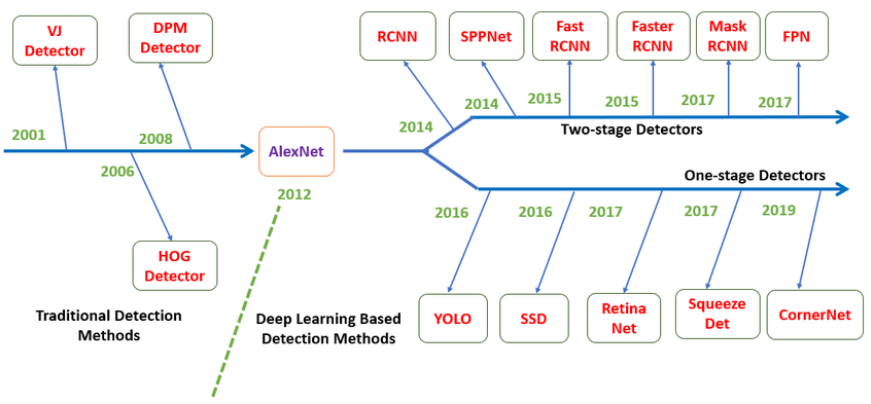
\includegraphics[width=0.7\textwidth]{images/Timeline.png}
    \caption{Timeline of Object Detection Methods}
    \label{fig:enter-label}
  \end{figure}
  % This block inserts a figure showing the timeline of object detection methods.
  % The 'label' command adds a reference to the figure that can be used elsewhere in the document. 
\end{itemize}
% This adds a new line and extra spacing after the list of methods.
%
% 1.3
{ \textbf{1.3 {YOLO (You Only Look Once)}}}\\\\
% This creates a new bolded heading for section "1.3 YOLO (You Only Look Once)".
% Double '\\' adds extra spacing after the section title.
%
YOLO is a family of single-stage object detection models recognized for their remarkable speed and accuracy. Unlike traditional two-stage detectors like Faster R-CNN, which first generate region proposals and then classify objects, YOLO simplifies the process by predicting bounding boxes and class probabilities in a single evaluation of the input image.
\\\newline
% This paragraph introduces YOLO and its key feature of using a single-stage detection process, compared to two-stage detectors like Faster R-CNN.
% '\\\newline' adds a new line and extra spacing after the paragraph.
%
\textbf{Key Features of YOLO: }
  \begin{itemize}
  \item \textbf{Unified Detection Process:} YOLO treats object detection as a single regression problem, directly predicting bounding boxes and class labels from the entire image in one step.
  \item \textbf{Real-Time Object Detection:} YOLO is optimized for speed, capable of performing real-time object detection with high frame rates, making it ideal for applications such as video analysis and autonomous systems.
  \item \textbf{End-to-End Optimization:} The entire YOLO pipeline is a single neural network, enabling end-to-end training and optimization, which contributes to improved detection performance.
  \item \textbf{High Accuracy:} YOLO models are known for their competitive accuracy on standard object detection benchmarks.
  \\
  \end{itemize}
% This block creates an itemized list of YOLO's key features, each of which is bolded and explained.
% '\item' is used to introduce each feature, and '\textbf' bolds the feature name.
% The '\\' adds a new line and extra spacing after the list.
%
% 1.4
{ \textbf{1.4 {Why YOLO}}}\\\\
% This creates a new bolded heading for section "1.4 Why YOLO".
% Double '\\' adds extra spacing after the section title.
%
YOLO has gained widespread popularity in computer vision due to its unique advantages over alternative object detection methods. Its combination of speed, accuracy, and simplicity makes it an attractive choice for a variety of applications, from real-time video analysis to autonomous systems.\\\\\\\\
% This paragraph explains why YOLO is popular and widely used, mentioning its advantages in terms of speed, accuracy, and simplicity.
% The double '\\\\\\\\' adds extra spacing before the following content.
%
\textbf{Advantages of YOLO: }
  \begin{itemize}
  \item \textbf{Speed:} YOLO’s single-stage architecture allows for real-time object detection with high frame rates, often outperforming two-stage detectors like Faster R-CNN in terms of speed. This makes YOLO highly suitable for applications requiring fast processing, such as video analysis and autonomous driving.
  \item \textbf{Accuracy:} YOLO delivers competitive accuracy on various benchmarks, making it reliable for a wide range of object detection tasks.
  \item \textbf{Generalization:} YOLO is capable of learning generalized representations of objects, improving its robustness and accuracy across different datasets.
  \item \textbf{Simplicity:} YOLO’s end-to-end design simplifies implementation, making it faster and easier than complex models like Faster R-CNN and more accurate than traditional methods like HOG and DPM.
  \end{itemize}
% This block creates an itemized list of the advantages of using YOLO, with each advantage highlighted in bold and followed by a description.
% '\item' introduces each new item, and '\textbf' is used for bold text.
%
YOLO stands out from other object detection methods by using a single-stage process, predicting bounding boxes and class probabilities in one step, unlike two-stage methods like Faster R-CNN. It is significantly faster, making it ideal for real-time applications.\\\\
% This paragraph summarizes how YOLO differs from other methods, emphasizing the single-stage process and its speed.
% The double '\\\\' adds extra spacing before the next content.
%
YOLO also uses anchor boxes to detect objects of varying sizes and generalizes better across different datasets compared to traditional hand-crafted feature methods. Its end-to-end training optimizes the entire network at once, making YOLO faster, simpler, and more adaptable than other object detection techniques.\\\\
% This paragraph further explains YOLO's use of anchor boxes for detecting objects of different sizes and highlights its generalization ability.
% The double '\\\\' adds extra spacing before the following figure.
%
\begin{figure}[h!]
    \centering
    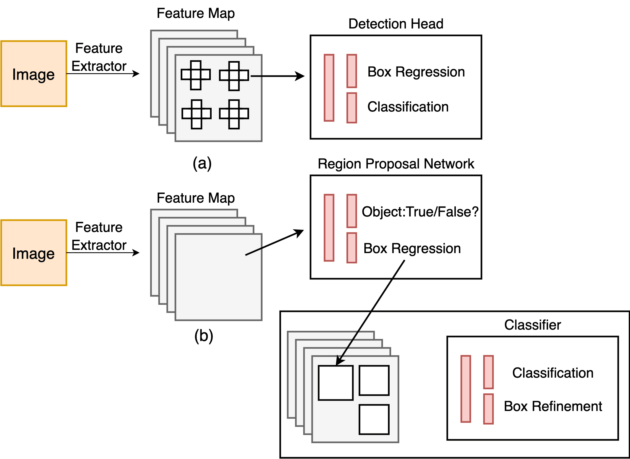
\includegraphics[width=0.7\textwidth]{images/1_vs_2 Stage.png}
    \caption{Single-Stage Detector vs Two-Stage Detector.}
\end{figure}
% This block inserts a figure that compares single-stage detectors (like YOLO) to two-stage detectors.
% '\centering' centers the figure horizontally on the page, and the 'width' option scales the image to 70% of the page width.
% '\caption' adds a description beneath the figure.
\\\\
% The double '\\\\' adds extra spacing before the next section.
%
% 1.5
{ \textbf{1.5 {How YOLO Works}}}\\\\
% This creates a new bolded heading for section "1.5 How YOLO Works".
% Double '\\' adds extra spacing after the section title.
%
YOLO is known for its innovative approach to object detection, offering both high speed and accuracy. Below is a detailed explanation of how the YOLO algorithm works:
% This sentence introduces the "How YOLO Works" section and mentions YOLO's key strengths of speed and accuracy.
%
\begin{enumerate}
  \item \textbf{Image Resizing and Grid Division:} YOLO first resizes the input image to a fixed size (e.g., 416x416) for standardization and efficiency. It then splits the image into an S x S grid, where each grid cell is responsible for detecting objects whose centers fall within it.
  % This is the first step in the YOLO process: resizing the image and dividing it into an SxS grid. The text explains how each grid cell detects objects based on their centers.
  %  
  \item \textbf{Bounding Boxes:} Each grid cell predicts B bounding boxes and confidence scores, indicating the likelihood that the box contains an object. Anchor boxes are used to define fixed aspect ratios and scales, enabling the model to better handle objects of varying shapes and sizes.
  % This step describes how each grid cell predicts bounding boxes and their confidence scores. The explanation also introduces anchor boxes for handling different object sizes and shapes.
  %
  \item \textbf{Prediction Generation:} For each bounding box, YOLO predicts:
   \begin{itemize}
  \item \textbf{Coordinates (x, y, w, h): } Center coordinates relative to the grid cell and dimensions relative to the image.
  % This explains that YOLO predicts the center coordinates (x, y) and dimensions (w, h) of each bounding box.
  %  
  \item \textbf{Confidence Score:} Represents the likelihood of an object being present and the accuracy of the box.
  % This defines the confidence score, which indicates how likely the bounding box contains an object and how accurate it is.
  %  
  \item \textbf{Class Probabilities:} Each grid cell predicts class probabilities, conditioned on containing an object.
  % This step mentions that class probabilities are predicted for each bounding box, but only if the grid cell contains an object.
   \end{itemize}
  % This is a nested itemized list within step 3, detailing the specific predictions YOLO makes for each bounding box.
  %
  \item \textbf{Non-Maximum Suppression (NMS):} NMS is used to eliminate duplicate detections, refining the results without significantly affecting performance.
  % The final step explains how Non-Maximum Suppression (NMS) is used to remove duplicate bounding boxes and ensure only the best detections are kept.
\end{enumerate}
% This block uses an enumerated list to explain the steps in the YOLO process: resizing and grid division, bounding box prediction, and non-maximum suppression.
%
\begin{figure}[h!]
    \centering
    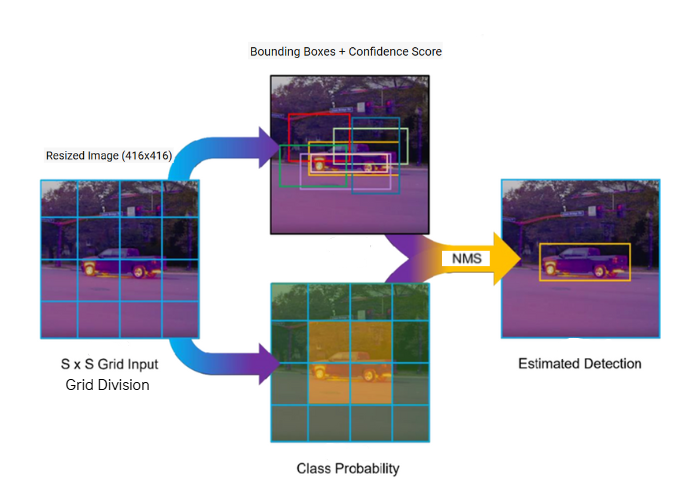
\includegraphics[width=0.7\textwidth]{images/Yolo Architecture.png}
    \caption{Working of YOLO}
\end{figure}
% This block inserts a figure showing the YOLO architecture.
% '\centering' centers the figure, and the 'width' option scales it to 70% of the page width.
% '\caption' adds a description below the figure.
%
% End of the chapter
%
%